%\documentclass[fleqn, letterpaper]{amsart}
\documentclass[fleqn, letterpaper]{tufte-handout}
\usepackage{times}
\usepackage{amsmath}
\usepackage{amssymb}
\usepackage{graphicx}
\usepackage{booktabs}
\usepackage{multirow}
\usepackage{listings}
\usepackage{epstopdf}
\usepackage{bm}
\usepackage{natbib}
%\usepackage[left=1in]{geometry}

\newcommand{\R}{\mathcal{R}}
\newcommand{\E}{\text{E}}
\newcommand{\p}{p_{XY}}
\newcommand{\T}{^\text{T}}
\renewcommand{\arraystretch}{1.5}

\title{Problem Set 4 --- ENCE689E Spring 2014}
\author{David Prentiss}

\begin{document}
\maketitle

\section{Time-varying (Dynamic) Model}

{\scriptsize
        \begin{minipage}{\linewidth}
                \lstinputlisting[language=Matlab, caption={Propagation of a linear soil moisture model},
                basicstyle=\ttfamily, label=lst1]{ps5a.m}
        \end{minipage}
}
\subsection{(b)}

\begin{figure}
        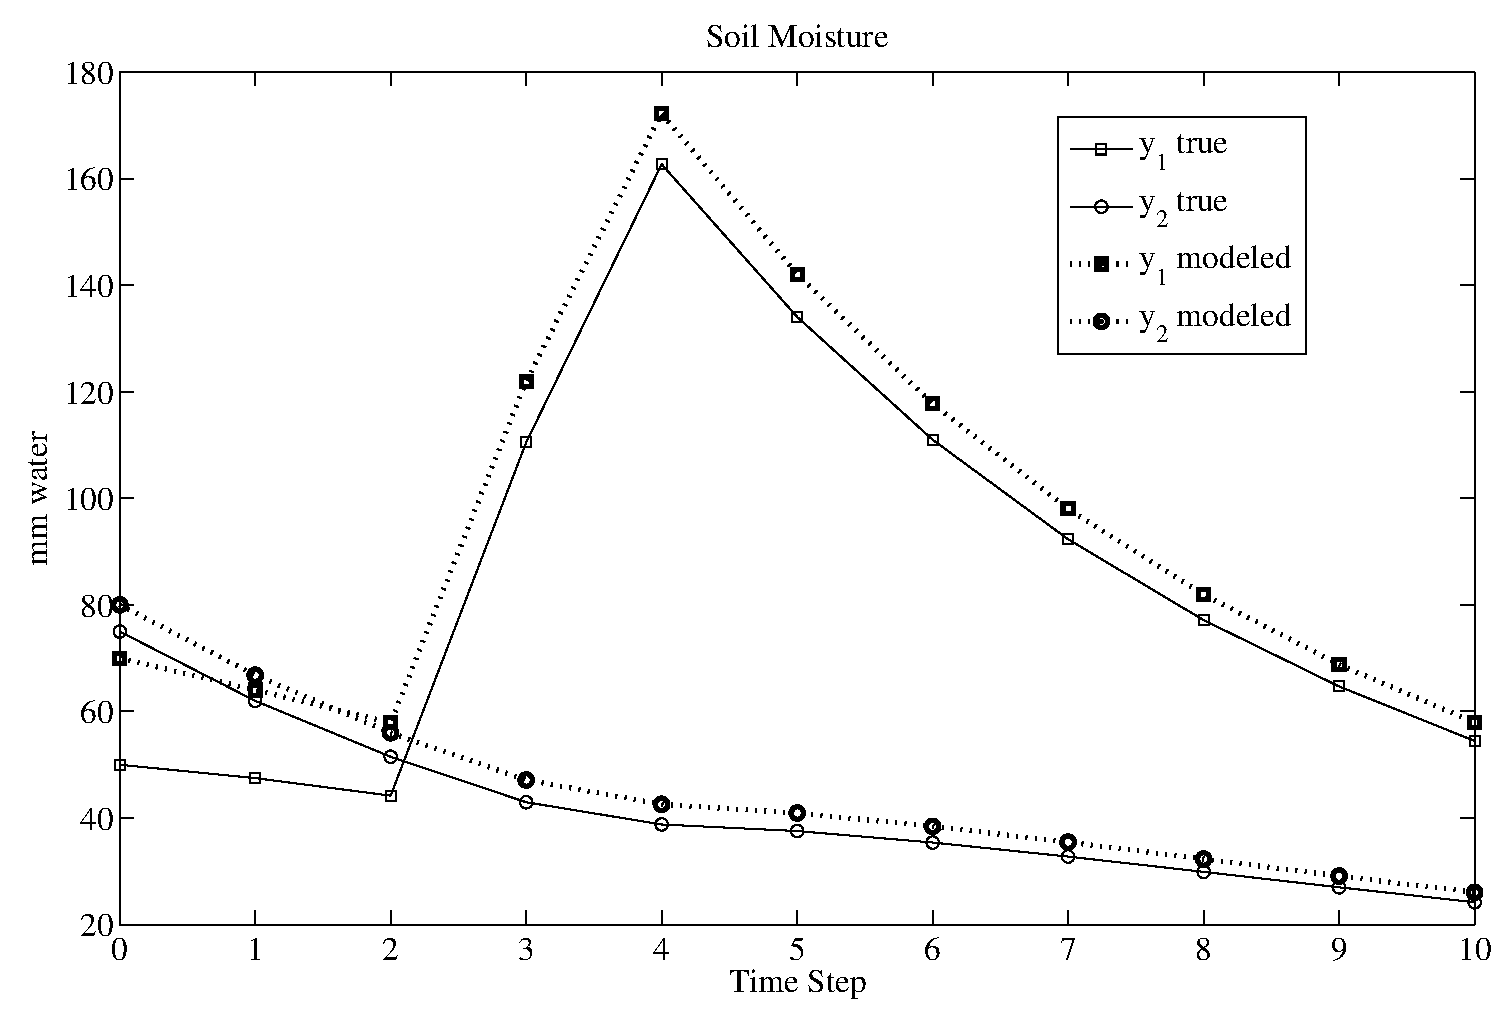
\includegraphics[width=\textwidth]{ps5figb}
        \caption{Deterministic estimate versus the true states}
        \label{ps5figb}
\end{figure}
See Figure \ref{ps5figb}. \emph{Including the initial conditions}, the temporally--averaged bias and root mean squared error are, respectively,
\[
        \begin{bmatrix}
                -9.4512 \\
                -3.4276
        \end{bmatrix}
        \text{ and }
        \begin{bmatrix}
                10.7630 \\
                3.5851
        \end{bmatrix}
\]

\subsection{(c)}
See Figure \ref{ps5figc}. \emph{Including the initial conditions}, the temporally--averaged bias and root mean squared error are the same as part (b), that is,
\[
        \begin{bmatrix}
                -9.4512 \\
                -3.4276
        \end{bmatrix}
        \text{ and }
        \begin{bmatrix}
                10.7630 \\
                3.5851
        \end{bmatrix}
\]
The expressions for the mean of the evolving pdf is
\[
        \bar{\mathbf{y}}_{t+1} = \mathbf{A}\bar{\mathbf{y}}_t + \mathbf{G}\bar{u}_t
\]
The evolving covariance is given by
\begin{align*}
        \mathbf{C}_{\mathbf{yy}}^{(t+1)} &= \mathbf{AC}_{\mathbf{yy}}^{(t)}\mathbf{A}^\intercal + \mathbf{GC}_\mathbf{{uu}}^{(t)}\mathbf{G}^\intercal \\
                                         & = \mathbf{AC}_{\mathbf{yy}}^{(t)}\mathbf{A}^\intercal + \mathbf{G}[0]\mathbf{G}^\intercal \\
                                         & = \mathbf{AC}_{\mathbf{yy}}^{(t)}\mathbf{A}^\intercal 
\end{align*}

\begin{figure}
        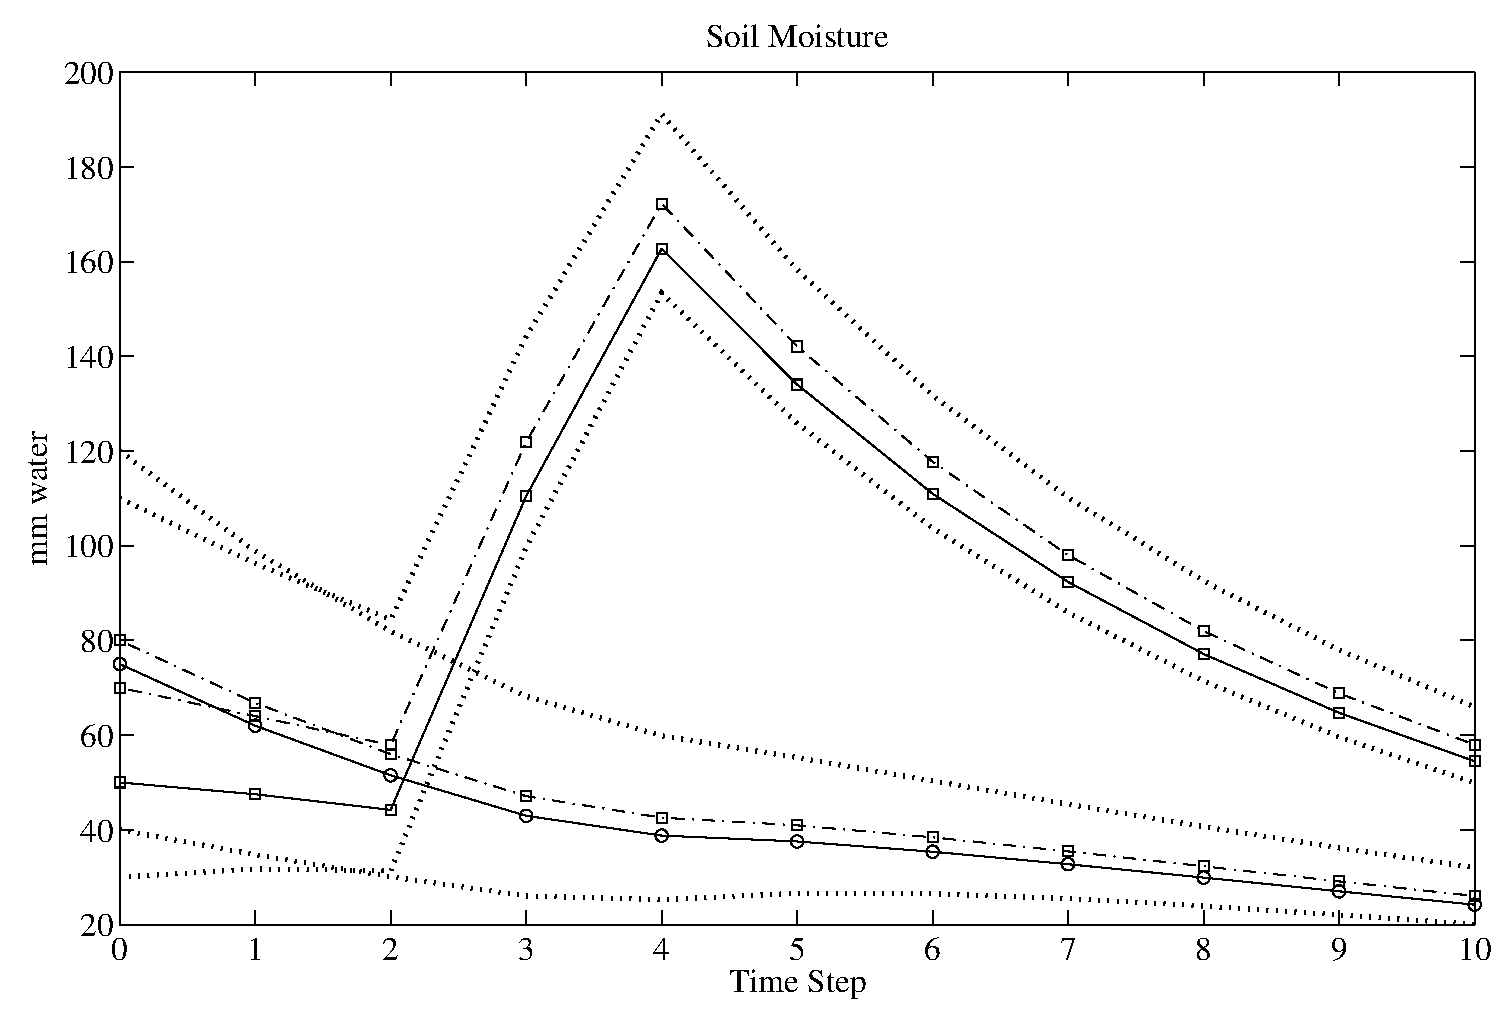
\includegraphics[width=\textwidth]{ps5figc}
        \caption{Deterministic estimate versus the true states with dotted lines indicating bounds on the estimates of two standard deviations.}
        \label{ps5figc}
\end{figure}

\subsection{(d)}
See Listing \ref{lst1}. The ensemble mean vector and covariance matrix for the initial conditions are, respectively, 
\[
        \begin{bmatrix}
                -69.7347 \\
                -81.5933
        \end{bmatrix}
        \text{ and }
        \begin{bmatrix}
                398.7850 & 5.0851 \\
                5.0851 & 443.0856
        \end{bmatrix}
\]

Since these values are generated with the mean and covariance of the estimate from part (b), we expect the ensemble mean and variance to be similar and approaching the estimate as the number of samples increase.

\subsection{(e)}

Because measurements of moisture are bound below at zero, a Gaussian distribution may not be the best to model the uncertainty of initial conditions. A disribution with a lower bound on its support would be more appropriate. Furthermore, since the probability of moistures close to zero should be decresing in the limit as the moisture approaches zero, a gamma distribution may be more appropriate.

\subsection{(f)}

As with the uncertainty in the initial conditions, the precipitation forcing is bound below at zero. An exponential ditsribution may be better. 

\subsection{(g)}

Since the model state mean vector $\bar{\mathbf{y}}_t$ is a Gaussian random vector, taking the coefficient matrix $\mathbf{A}$ to contain random variables would mean the transformation $\mathbf{A}\bar{\mathbf{y}}_t$ is no longer linear and the evolving pdf would not, in general be Gaussian.

\end{document}
